\documentclass[a4paper,12pt]{article}

\title{Chapter 3. The Dirac Field\\
3-6. Discrete Symmetries of the Dirac Theory}
\date{各種SNS\\
    X (旧 Twitter): \href{https://x.com/miya_max_study}{@miya\_max\_study}\\
    Instagram : \href{https://www.instagram.com/daily_life_of_miya/}{@daily\_life\_of\_miya}\\
    YouTube : \href{https://www.youtube.com/@miya-max-active}{@miya-max-active}
    }
\author{Max Miyazaki}

\usepackage{amsmath}
\usepackage{amssymb}
\usepackage{ascmac}
\usepackage{amsthm}
\usepackage{amsfonts}
\usepackage{enumitem}
\usepackage{color}
\usepackage[dvipdfmx]{graphicx}
\usepackage{float}
\usepackage{bm}
\usepackage{here}

% Define slashed notation
\newcommand{\slashed}[1]{\not{#1}}

\usepackage{abstract}
\usepackage{tikz}
\usetikzlibrary{shapes.geometric, arrows.meta, positioning}
\usepackage{indentfirst}
\usepackage[utf8]{inputenc}
\usepackage{fix-cm}
\usepackage{wrapfig}
\pagenumbering{arabic}
\usepackage{url}
\usepackage{xcolor}
\usepackage[most]{tcolorbox}
\usepackage{framed}
\usepackage[dvipdfmx]{hyperref}
\hypersetup{
 setpagesize=false,
 bookmarksnumbered=true,
 colorlinks=true,
 linkcolor=blue
}

% Define braket-like commands
\newcommand{\bra}[1]{\left\langle #1\right|}
\newcommand{\ket}[1]{\left|#1\right\rangle}
\newcommand{\braket}[2]{\left\langle #1\middle|#2\right\rangle}
\newcommand{\brakets}[3]{\left\langle #1\middle| #2 \middle|#3 \right\rangle}

\renewcommand{\arraystretch}{2.1}


\setlength{\textwidth}{16cm}
\setlength{\textheight}{25cm}
\setlength{\oddsidemargin}{0cm}
\setlength{\evensidemargin}{0cm}
\setlength{\topmargin}{-2cm}

\begin{document}
\maketitle

\vspace{1cm}
\begin{abstract}
    このノートはPeskin\&Schroederの``An Introduction to Quantum Field Theory''の第3章の5節をまとめたものである. 要点や個人的な追記, 計算ノート的なまとめを行っているが, それらはすべて原書の内容を出発点としている. 参考程度に使っていただきたいが, このノートは私の勉強ノートであり, そのままの内容をそのまま鵜呑みにすると間違った理解を招く可能性があることをご了承ください. ぜひ原著を手に取り, その内容をご自身で確認していただくことを推奨します. てへぺろ v$({\hat{\cdot}_\partial \hat{\cdot}})$v
\end{abstract}
    
    

\newpage
\color{blue}
\section*{概要}

\begin{itemize}
  \item \textbf{対象とする3つの離散対称性}
  \begin{itemize}
    \item パリティ ($P$): $(t,\mathbf{x}) \to (t,-\mathbf{x})$
    \item 時間反転 ($T$): $(t,\mathbf{x}) \to (-t,\mathbf{x})$
    \item 電荷共役 ($C$): 粒子と反粒子を入れ替える
  \end{itemize}
  \item これらはいずれも $x^2=t^2-\mathbf{x}^2$ を保存する.
  \item 実験事実:
  \begin{itemize}
    \item 重力・電磁気力・強相互作用は $C,P,T$ に対称.
    \item 弱相互作用は $C,P$ を破るが $CP$ と $T$ は保存.
    \item 中性K中間子の稀な過程では $CP$ および $T$ の破れが観測される.
    \item すべての観測は $CPT$ が完全な対称性であることを示す.
  \end{itemize}

  \item \textbf{パリティ $P$}
  \begin{itemize}
    \item 場の変換: $P\psi(t,\mathbf{x})P = \eta_a \gamma^0 \psi(t,-\mathbf{x})$.
    \item 双線形の変換:
    \begin{itemize}
      \item $\bar{\psi}\psi$: 偶パリティ
      \item $\bar{\psi}\gamma^\mu\psi$: $\mu=0$ 成分は偶, $\mu=1,2,3$ 成分は奇
      \item $i\bar{\psi}\gamma^5\psi$: 奇パリティ
      \item $\bar{\psi}\gamma^\mu\gamma^5\psi$: $\mu=0$ 成分は奇, 空間成分は偶
    \end{itemize}
    \item フェルミオン–アンチフェルミオン対は $P$ で固有値 $-1$.
    \item 束縛状態のパリティ則:
    \begin{itemize}
      \item 空間波動関数が対称なら奇パリティ, 反対称なら偶パリティ.
      \item $L=0$ 束縛状態は奇パリティ.
      \item $J=0$ 状態は擬スカラー, $J=1$ 状態はベクトルとして変換.
    \end{itemize}
  \end{itemize}

  \item \textbf{時間反転 $T$}
  \begin{itemize}
    \item $T$ は線形ユニタリではなく反ユニタリ演算子.
    \item スピン反転を伴う: $\xi^s \to \xi^{s*}=-i\sigma^2(\xi^s)^*$.
    \item 場の変換: $T\psi(t,\mathbf{x})T=(\gamma^1\gamma^3)\psi(-t,\mathbf{x})$.
    \item 双線形の変換:
    \begin{itemize}
      \item スカラー: 不変
      \item 擬スカラー: マイナス符号を得る
      \item ベクトル: $\mu=0$ 成分は偶, 空間成分は奇
    \end{itemize}
  \end{itemize}

  \item \textbf{電荷共役 $C$}
  \begin{itemize}
    \item 消滅演算子の変換: $Ca^s_{\mathbf{p}}C=b^s_{\mathbf{p}}, \quad Cb^s_{\mathbf{p}}C=a^s_{\mathbf{p}}$.
    \item 場の変換: $C\psi(x)C=-i\gamma^2\psi^*(x)$.
    \item 双線形の変換:
    \begin{itemize}
      \item $\bar{\psi}\psi$: 不変
      \item $i\bar{\psi}\gamma^5\psi$: 不変
      \item $\bar{\psi}\gamma^\mu\psi$: 符号反転
      \item $\bar{\psi}\gamma^\mu\gamma^5\psi$: 不変
    \end{itemize}
  \end{itemize}

  \item \textbf{$C,P,T$ のまとめ}
  \begin{itemize}
    \item 自由ディラック・ラグランジアン
    \[
    \mathcal{L}_0=\bar{\psi}(i\gamma^\mu\partial_\mu-m)\psi
    \]
    は $C,P,T$ のそれぞれに対して不変.
    \item 一般に, ローレンツ不変かつエルミートな量子場理論は常に $CPT$ 対称性を満たす.
  \end{itemize}
\end{itemize}


\newpage
\color{black}
\section*{3.6 Discrete Symmetries of the Dirac Theory}

前節では, Dirac 理論の Hilbert 空間における連続 Lorentz 変換の実装について議論した.  
各変換 $\Lambda$ に対してユニタリ演算子 $U(\Lambda)$ が存在し, それは場に対して
\begin{equation}
U(\Lambda)\psi(x)U^{-1}(\Lambda) = \Lambda^{-1}_{1/2}\psi(\Lambda x)
\tag{3.122}
\end{equation}
という正しい変換を誘導した.

本節では, Dirac 場に対して種々の \textbf{離散対称性} を実装する演算子を議論する.  

連続 Lorentz 変換に加えて, Lagrangian の対称性である可能性をもつ時空操作が二つ存在する:  
\textbf{空間反転 (Parity)} と \textbf{時間反転 (Time reversal)} である.  

- Parity $P$: $(t,\mathbf{x}) \to (t,-\mathbf{x})$, 空間の向きを反転させる.  
- 時間反転 $T$: $(t,\mathbf{x}) \to (-t,\mathbf{x})$, 光円錐の前向き・後向きを入れ替える.  

これらはいずれも恒等変換から連続 Lorentz 変換で実現することはできない.  
しかし両者とも Minkowski 間隔 $x^2=t^2-\mathbf{x}^2$ を保存する.  

標準的な呼び方では, 連続 Lorentz 変換は「正の向きの直交 Lorentz 群」 $L_+^\uparrow$ と呼ばれる.  
完全な Lorentz 群は, 以下のように不連続な部分群に分解される:

\begin{figure}[H]
\begin{center}
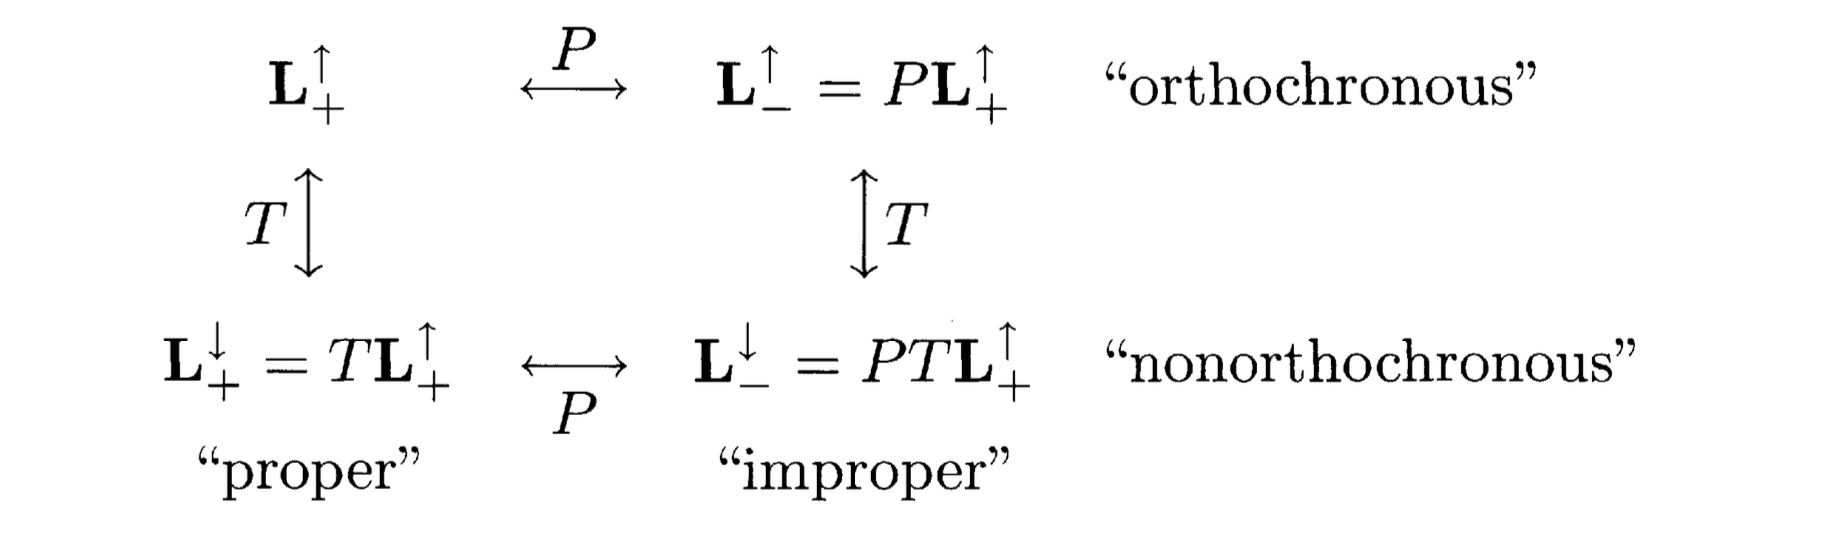
\includegraphics[scale=0.4]{figures/Lorentz_group.png}
\end{center}
\end{figure}

ここで, $L_+^\uparrow$ は「proper」, $L_-^\downarrow$ は「improper」と呼ばれる.

$P$ や $T$ と同時に, 便宜上, 三つ目の(時空ではない)離散操作 \textbf{電荷共役 (charge conjugation)} $C$ を導入する.  
この操作の下では粒子と反粒子が入れ替わる.

一般に相対論的場の理論は $P$, $T$, $C$ に対して不変である必要はない.  
実際の世界ではどうだろうか?  

- 実験から, 自然界の4つの力のうち, 重力・電磁気力・強い相互作用は $P,C,T$ のすべてに対して対称であることが知られている.  
- しかし弱い相互作用は $C$ と $P$ をそれぞれ破るが, $CP$ と $T$ は保存する.  
- ところが希な過程(中性 $K$ 中間子に関わるもの)は $CP$ と $T$ の破れを示す.  
- すべての観測は, 組み合わせ $CPT$ が完全な対称性であることを示している.

現在広く受け入れられている弱い相互作用の理論モデルは, Glashow-Weinberg-Salam model である.  
この理論は $C$ と $P$ を最も強い形で破る.  
驚くべきことに(偶然ではないかもしれないが), $C$ と $P$ は最も観測しやすい過程ではよい対称性として現れる.  
一方で, 本当に美しい $CP$ 対称を破る理論は未だ知られていない.  

現在の理論では, Fermion 世代が3つ (またはそれ以上) ある場合, あるパラメータが非ゼロであれば $CP$ 破れが生じうる.  
しかしこのパラメータの値は電子質量と同程度にしか理解されておらず, $CP$ 破れの物理的起源は依然として謎である.  

この問題については第20.3節でさらに議論する.

\subsubsection*{Parity}

ここで $P,T,C$ の作用を Dirac 粒子や場について議論しよう.  
まず Parity を考える. Parity 演算子 $P$ は粒子の運動量を反転させ, スピンを保持するはずである:

\[
\text{mirror:} \quad \mathbf{p} \to -\mathbf{p}
\]

数学的には, Parity はユニタリ演算子(正確には $U(P)$, ここでは $P$ と書く)として実装され,  
例えば生成演算子を
\begin{equation}
P a^s_{\mathbf{p}} P = \eta_a a^s_{\bar{\mathbf{p}}}, 
\qquad 
P b^{s\dagger}_{\mathbf{p}} P = \eta_b b^{s\dagger}_{\bar{\mathbf{p}}}
\tag{3.123}
\end{equation}
のように変換する. ここで $\eta_a,\eta_b$ は位相因子である.  

これらは $P^2=1$ であることから $\eta_a^2=\eta_b^2=\pm1$ の制限を受ける.  

連続 Lorentz 変換が Dirac 場に $4\times4$ の行列として作用するのと同様に,  
Parity 変換も $4\times4$ の行列で表されるべきである.  
式 (3.123) を $\psi(x)$ の展開に適用すると,
\begin{equation}
P\psi(t,\mathbf{x})P = \int \frac{d^3p}{(2\pi)^3}\frac{1}{\sqrt{2E_p}}
\sum_s \left( \eta_a a^s_{\bar{\mathbf{p}}} u^s(p) e^{-ip\cdot x}
+ \eta_b b^{s\dagger}_{\bar{\mathbf{p}}} v^s(p) e^{ip\cdot x} \right).
\tag{3.124}
\end{equation}

ここで $\bar{p}=(p^0,-\mathbf{p})$.  
スピノルは
\begin{align*}
u(p) &= \begin{pmatrix} \sqrt{p\cdot\sigma}\,\xi \\ \sqrt{p\cdot\bar\sigma}\,\xi \end{pmatrix},
\quad
u(\bar{p}) = \gamma^0 u(p), \\
v(p) &= \begin{pmatrix} \sqrt{p\cdot\sigma}\,\eta \\ -\sqrt{p\cdot\bar\sigma}\,\eta \end{pmatrix},
\quad
v(\bar{p}) = -\gamma^0 v(p),
\end{align*}
である. よって
\begin{equation}
P\psi(x)P = \int \frac{d^3p}{(2\pi)^3}\frac{1}{\sqrt{2E_p}}
\sum_s \left( \eta_a \gamma^0 u^s(\bar{p}) a^s_{\bar{\mathbf{p}}} e^{-ip\cdot x}
- \eta_b \gamma^0 v^s(\bar{p}) b^{s\dagger}_{\bar{\mathbf{p}}} e^{ip\cdot x} \right).
\tag{3.125}
\end{equation}

最終的に, Parity 変換は
\begin{equation}
P\psi(t,\mathbf{x})P = \eta_a \gamma^0 \psi(t,-\mathbf{x})
\tag{3.126}
\end{equation}
となる.

Lagrangian を書き下す際には, Dirac 場の双線形形式の変換性が重要である.  
5種類の双線形は
\begin{equation}
\bar{\psi}\psi, \quad \bar{\psi}\gamma^\mu\psi, \quad 
i\bar{\psi}\gamma^5\psi, \quad 
\bar{\psi}\gamma^\mu\gamma^5\psi, \quad 
\bar{\psi}\sigma^{\mu\nu}\psi
\tag{3.127}
\end{equation}
である.

- スカラー項:
\begin{equation}
P\bar{\psi}\psi P = \eta_a^2 \bar{\psi}(t,-\mathbf{x})\psi(t,-\mathbf{x})
= +\bar{\psi}\psi(t,-\mathbf{x})
\tag{3.129}
\end{equation}

- ベクトル項:
\begin{equation}
P\bar{\psi}\gamma^\mu\psi P =
\begin{cases}
+\bar{\psi}\gamma^0\psi(t,-\mathbf{x}), & \mu=0, \\
-\bar{\psi}\gamma^i\psi(t,-\mathbf{x}), & \mu=1,2,3,
\end{cases}
\tag{3.130}
\end{equation}
空間成分に符号反転がかかる.

- 擬スカラー・擬ベクトル項:
\begin{align}
P i\bar{\psi}\gamma^5\psi P &= -i\bar{\psi}\gamma^5\psi(t,-\mathbf{x}),
\tag{3.131} \\
P \bar{\psi}\gamma^\mu\gamma^5\psi P &=
\begin{cases}
-\bar{\psi}\gamma^0\gamma^5\psi(t,-\mathbf{x}), & \mu=0, \\
+\bar{\psi}\gamma^i\gamma^5\psi(t,-\mathbf{x}), & \mu=1,2,3.
\end{cases}
\tag{3.132}
\end{align}

前節 3.4 で予想したように, 「擬 (pseudo)」は Parity 変換における余分なマイナス符号を意味する.  
(双線形 $\bar{\psi}[\gamma^\mu,\gamma^\nu]\psi = 2i\bar{\psi}\sigma^{\mu\nu}\psi$ の変換性については問題 3.7 で扱う.)  
Fermion の双線形の変換性は $\eta_a$ に依存しないので, 一般性を失うことなく最初から $\eta_a=-\eta_b=1$ と置ける.  

しかし, Fermion と anti-Fermion の Parity 変換の間の相対的なマイナス符号 (式 3.125) は重要な意味をもつ.  
例えば Fermion–anti-Fermion 対の状態 $a^{s\dagger}_{\mathbf{p}} b^{t\dagger}_{\mathbf{q}}|0\rangle$ を考える.  
Parity を作用させると
\[
P\left(a^{s\dagger}_{\mathbf{p}} b^{t\dagger}_{\mathbf{q}}|0\rangle\right) 
= -(a^{s\dagger}_{\bar{\mathbf{p}}} b^{t\dagger}_{\bar{\mathbf{q}}}|0\rangle).
\]
したがって, Fermion–anti-Fermion 対を含む状態は Parity で固有値 $-1$ を得る.  

この情報は束縛状態の文脈で特に有用である. すなわち, Fermion と anti-Fermion の運動量を Schrödinger 波動関数で重ね合わせ, 空間に局在した系を構成するときである.  

このような状態については第5.3節で詳しく扱うが, ここで次を指摘しておこう.  

- 空間波動関数が $\mathbf{x}\to-\mathbf{x}$ に対して対称なら, 状態は \textbf{odd parity} をもつ.  
- 空間波動関数が $\mathbf{x}\to-\mathbf{x}$ に対して反対称なら, 状態は \textbf{even parity} をもつ.  

具体的には:  
- $L=0$ の束縛状態は odd parity をもつ.  
- $J=0$ の状態は擬スカラーとして変換する.  
- $J=1$ の3つの状態はベクトルの空間成分として変換する.  

これらの性質は, 陽電子やクォーク–反クォーク系の崩壊における選択則に現れる (問題 3.8 参照).

\subsubsection*{Time Reversal}

次に時間反転の実装について議論する.  
我々は $T$ をユニタリ演算子として, $a_{\mathbf{p}} \to a_{-\mathbf{p}}$ ($b_{\mathbf{p}}$ についても同様),  
$\psi(t,\mathbf{x}) \to \psi(-t,\mathbf{x})$(行列因子付き)を実現させたい.  

しかしこれは非常に困難である.  
というのも, 展開式で $(t,\mathbf{x}) \to (-t,\mathbf{x})$ としたとき, $a_{\mathbf{p}} \to a_{-\mathbf{p}}$ だけでは不十分だからである.  
特に, 自由 Dirac 理論の対称性条件 $[T,H]=0$ を課すと困難さが顕著になる.  

\begin{equation*}
\psi(t,\mathbf{x}) = e^{iHt}\psi(0,\mathbf{x})e^{-iHt}
\end{equation*}

これに $T$ を作用させると
\begin{align*}
T\psi(t,\mathbf{x})T &= e^{iHt}[T\psi(0,\mathbf{x})T] e^{-iHt}, \\
\Rightarrow T\psi(t,\mathbf{x})T|0\rangle &= e^{iHt}[T\psi(0,\mathbf{x})T]|0\rangle.
\end{align*}

ここで $H|0\rangle=0$ を仮定した.  
右辺は負の周波数成分だけの和になってしまう.  
一方 $T$ が $\psi(t,\mathbf{x})$ の時間依存を反転させるのであれば, 左辺は $\psi(-t,\mathbf{x})|0\rangle=e^{-iHt}\psi(0,\mathbf{x})|0\rangle$ となり, 正の周波数成分だけから成る.  

したがって, $T$ は線形ユニタリ演算子としては実装できない.  

ではどうするか?  
解決策は, $T^\dagger=T^{-1}$ を満たしつつ, $T$ が $c$ 数に作用する際には複素共役を伴うように定義することである:
\begin{equation}
T(c\text{-number}) = (c\text{-number})^* T.
\tag{3.133}
\end{equation}

このとき $[T,H]=0$ でも, すべての指数因子 $e^{-iHt}$ は $e^{+iHt}$ に反転する.  
量子力学では時間発展は常にこの形の指数因子で表されるので, これは事実上 $t$ の符号を反転させることになる.  

ここで $T$ は非線形演算子(正確には \textbf{反線形 (antilinear)} または \textbf{反ユニタリ (antiunitary)} 演算子)であることに注意.  

また, 運動量を反転させるのに加え, 時間反転 $T$ はスピンも反転させる必要がある.  

スピノル $\xi$ のスピンを反転させる数学的操作を見つけよう.  
章の前半ではスピン状態をラベル $s=1,2$ で表したが, 以降はスピンの向きを特定の軸に沿って表す.  

もしスピンの軸が極座標 $\theta,\phi$ で与えられているなら, スピンアップ・スピンダウンの2成分スピノルは
\begin{equation*}
\xi(\uparrow)=\begin{pmatrix}\cos \tfrac{\theta}{2} \\ e^{i\phi}\sin\tfrac{\theta}{2}\end{pmatrix}, \quad
\xi(\downarrow)=\begin{pmatrix}-e^{-i\phi}\sin\tfrac{\theta}{2} \\ \cos\tfrac{\theta}{2}\end{pmatrix}.
\end{equation*}

スピン反転スピノルを
\begin{equation}
\xi^{s*} = -i\sigma^2 (\xi^s)^*
\tag{3.134}
\end{equation}
と定義すると,
\begin{equation}
\xi^{s*}=(\xi(\downarrow),-\xi(\uparrow))
\tag{3.135}
\end{equation}
となる.  

このスピン反転の関係は恒等式 $\sigma^2\sigma^i\sigma^2=-(\sigma^i)^*$ から導かれる.  
したがって, $\xi$ が $\mathbf{n}\cdot\sigma \,\xi=\pm\xi$ を満たすなら,
\begin{equation*}
\mathbf{n}\cdot\sigma (-i\sigma^2 \xi^*)=-i\sigma^2(\mathbf{n}\cdot\sigma)^*\xi^*=-(\mathbf{n}\cdot\sigma)(-i\sigma^2\xi^*).
\end{equation*}
つまり2回スピン反転を行うと $-1$ がかかり, 元の状態に戻る.  

電子の消滅演算子 $a^s_{\mathbf{p}}$ はスピノル $u^s(p)$ を含む.  
陽電子の消滅演算子 $b^s_{\mathbf{p}}$ はスピノル $v^s(p)$ を含む.  

ここで
\begin{equation}
v^s(p) = \begin{pmatrix}\sqrt{p\cdot\sigma}\,\xi^{s*} \\ -\sqrt{p\cdot\bar\sigma}\,\xi^{s*}\end{pmatrix}
\tag{3.136}
\end{equation}
とおき, また
\begin{equation}
a^{s*}_{\mathbf{p}}=(a^2_{\mathbf{p}},-a^1_{\mathbf{p}}), \quad
b^{s*}_{\mathbf{p}}=(b^2_{\mathbf{p}},-b^1_{\mathbf{p}})
\tag{3.137}
\end{equation}
と定義する.  

Dirac スピノル $u, v$ とその時間反転の関係を導こう.  
$\tilde{p}=(p^0,-\mathbf{p})$ と定義する.  
このベクトルは恒等式
\begin{equation*}
\sqrt{\tilde{p}\cdot\sigma}\,\sigma^2 = \sigma^2 \sqrt{p\cdot\sigma^*}
\end{equation*}
を満たす. (これを証明するには, (3.49) のように平方根を展開すればよい.)

あるスピンと運動量の選択に対して, Dirac スピノル $u^s(p)$ に対応する $\tilde{p}$ のスピノルを $u^{-s}(\tilde{p})$ とすると,  
両者は次のように関係する:
\begin{align*}
u^{-s}(\tilde{p}) &=
\begin{pmatrix}
\sqrt{\tilde{p}\cdot\sigma}(-i\sigma^2 \xi^{s*}) \\
\sqrt{\tilde{p}\cdot\bar\sigma}(-i\sigma^2 \xi^{s*})
\end{pmatrix} \\
&=
\begin{pmatrix}
- i\sigma^2 \sqrt{p\cdot\sigma^*}\,\xi^{s*} \\
- i\sigma^2 \sqrt{p\cdot\bar\sigma^*}\,\xi^{s*}
\end{pmatrix} \\
&= -i
\begin{pmatrix}
\sigma^2 & 0 \\ 0 & \sigma^2
\end{pmatrix}[u^s(p)]^* \\
&= -\gamma^1\gamma^3 [u^s(p)]^* .
\end{align*}

同様に $v^s(p)$ についても
\begin{equation*}
v^{-s}(\tilde{p}) = -\gamma^1\gamma^3 [v^s(p)]^* .
\end{equation*}

この関係において, $v^{-s}$ は $\xi^{-s}=-\xi^s$ を含む.

式 (3.137) の記法を用いると, Fermion 消滅演算子の時間反転変換は次のように定義される:
\begin{equation}
Ta^s_{\mathbf{p}}T = a^{-s}_{\bar{\mathbf{p}}}, 
\qquad 
Tb^s_{\mathbf{p}}T = b^{-s}_{\bar{\mathbf{p}}}.
\tag{3.138}
\end{equation}
(全体の位相因子は以降の議論には影響しないため省略した.)

これにより, Fermion 場 $\psi(x)$ に対する $T$ の作用を計算できる:
\begin{align*}
T\psi(t,\mathbf{x})T 
&= \int \frac{d^3p}{(2\pi)^3}\frac{1}{\sqrt{2E_p}}
\sum_s T\Big( a^s_{\mathbf{p}} u^s(p)e^{-ipx} + b^{s\dagger}_{\mathbf{p}} v^s(p)e^{ipx} \Big) T \\
&= \int \frac{d^3p}{(2\pi)^3}\frac{1}{\sqrt{2E_p}}
\sum_s \left( a^{-s}_{\bar{\mathbf{p}}}[u^s(p)]^* e^{ipx}
+ b^{-s\dagger}_{\bar{\mathbf{p}}}[v^s(p)]^* e^{-ipx} \right) \\
&= (\gamma^1\gamma^3)\int \frac{d^3\tilde{p}}{(2\pi)^3}\frac{1}{\sqrt{2E_{\tilde{p}}}}
\sum_s \Big( a^{-s}_{\tilde{\mathbf{p}}}u^{-s}(\tilde{p})e^{i\tilde{p}\cdot(t,-\mathbf{x})} \\
&\hspace{4cm}
+ b^{-s\dagger}_{\tilde{\mathbf{p}}} v^{-s}(\tilde{p})e^{-i\tilde{p}\cdot(t,-\mathbf{x})} \Big) \\
&= (\gamma^1\gamma^3)\psi(-t,\mathbf{x}).
\tag{3.139}
\end{align*}

最後のステップでは, $\tilde{p}=(p^0,-\mathbf{p})$ を用いた.  
Parity の場合と同様に, $\psi(x)$ に対して単純な変換則が得られた.  
相対的なマイナス符号は, 粒子と反粒子の変換法則に含まれており, また $v^{-s}$ のスピノルを2回反転したことにも反映されている.

次に, 双線形に対する $T$ の作用を確認する.  
まず
\begin{equation*}
T\bar{\psi}T = (T\psi T)^\dagger(\gamma^0)^* 
= \psi^\dagger(-t,\mathbf{x})[\gamma^1\gamma^3]^\dagger\gamma^0 
= \bar{\psi}(-t,\mathbf{x})[-\gamma^1\gamma^3].
\tag{3.140}
\end{equation*}

したがってスカラー双線形の変換は
\begin{equation*}
T\bar{\psi}\psi(t,\mathbf{x})T 
= \bar{\psi}(-t,\mathbf{x})(-\gamma^1\gamma^3)(\gamma^1\gamma^3)\psi(-t,\mathbf{x}) 
= +\bar{\psi}\psi(-t,\mathbf{x}).
\tag{3.141}
\end{equation*}

擬スカラーは, $T$ が $i$ を通過する際に余分なマイナス符号を得る:
\begin{equation*}
T i\bar{\psi}\gamma^5\psi T 
= -i\bar{\psi}(-\gamma^1\gamma^3)\gamma^5(\gamma^1\gamma^3)\psi 
= -i\bar{\psi}\gamma^5\psi(-t,\mathbf{x}).
\end{equation*}

ベクトルの場合, 各成分 $\mu=0,1,2,3$ ごとに計算が必要であり, 結果は以下となる:
\begin{equation*}
T\bar{\psi}\gamma^\mu\psi T 
= \bar{\psi}(-\gamma^1\gamma^3)(\gamma^\mu)^*(\gamma^1\gamma^3)\psi
= 
\begin{cases}
+\bar{\psi}\gamma^0\psi(-t,\mathbf{x}), & \mu=0, \\
-\bar{\psi}\gamma^i\psi(-t,\mathbf{x}), & \mu=1,2,3,
\end{cases}
\tag{3.142}
\end{equation*}

これは電流のようなベクトルに期待される変換性と一致する.  
同様に, 擬ベクトルも正しく変換されることが確認できる.

\subsubsection*{Charge Conjugation}

3つの離散対称性の最後は粒子–反粒子対称性 $C$ である.  
$C$ はユニタリ線形演算子として問題なく実装できる.  
電荷共役は, 与えられたスピン方向をもつ Fermion を, 同じスピン方向をもつ anti-Fermion に変換する操作として定義される.  
したがって消滅演算子の変換として便利な選択は
\begin{equation*}
C a^s_{\mathbf{p}} C = b^s_{\mathbf{p}}, 
\qquad 
C b^s_{\mathbf{p}} C = a^s_{\mathbf{p}} .
\tag{3.143}
\end{equation*}
(簡単のため全体位相は無視する.)

次に, $\psi(x)$ に対する $C$ の作用を計算する.  
$v^s(p)$ と $u^s(p)$ の関係が必要となる.  
式 (3.136) と (3.134) を用いると
\begin{equation*}
(v^s(p))^* = 
\begin{pmatrix}
\sqrt{p\cdot\sigma}(-i\sigma^2\xi^{s*}) \\
-\sqrt{p\cdot\bar\sigma}(-i\sigma^2\xi^{s*})
\end{pmatrix}^*
= \begin{pmatrix}
0 & -i\sigma^2 \\ i\sigma^2 & 0
\end{pmatrix}
\begin{pmatrix}
\sqrt{p\cdot\sigma}\,\xi \\ \sqrt{p\cdot\bar\sigma}\,\xi
\end{pmatrix}.
\end{equation*}

すなわち
\begin{equation}
u^s(p) = -i\gamma^2 (v^s(p))^*, 
\qquad 
v^s(p) = -i\gamma^2 (u^s(p))^* .
\tag{3.144}
\end{equation}

これを Fermion 場の展開式に代入し, $C$ を作用させると
\begin{align*}
C\psi(x)C &= \int \frac{d^3p}{(2\pi)^3}\frac{1}{\sqrt{2E_p}}
\sum_s \Big( -i\gamma^2 b_{\mathbf{p}}^s (v^s(p))^* e^{-ipx}
- i\gamma^2 a_{\mathbf{p}}^{s\dagger}(u^s(p))^* e^{ipx} \Big) \\
&= -i\gamma^2 \psi^*(x) 
= -i\gamma^2 (\psi^\dagger)^T 
= -i (\bar{\psi}\gamma^0\gamma^2)^T.
\tag{3.145}
\end{align*}

したがって $C$ は $\psi\to\psi^*$ とするが, ユニタリ線形演算子である.

次に双線形に対する $C$ の作用を調べる. まず
\begin{equation*}
C\bar{\psi}(x)C = C\psi^\dagger C \gamma^0 = (-i\gamma^2\psi)^T\gamma^0 
= (-i\gamma^0\gamma^2\psi)^T.
\tag{3.146}
\end{equation*}

スカラーの場合:
\begin{align*}
C\bar{\psi}\psi C &= (-i\gamma^0\gamma^2\psi)^T(-i\bar{\psi}\gamma^0\gamma^2)^T \\
&= -\bar{\psi}\gamma^2\gamma^0\gamma^0\gamma^2\psi \\
&= +\bar{\psi}\psi.
\tag{3.147}
\end{align*}
(第3行のマイナス符号は反交換のため.)

擬スカラーの場合:
\begin{equation*}
C i\bar{\psi}\gamma^5\psi C 
= i(-i\gamma^0\gamma^2\psi)^T \gamma^5 (-i\bar{\psi}\gamma^0\gamma^2)^T
= i\bar{\psi}\gamma^5\psi.
\tag{3.148}
\end{equation*}

ベクトル・擬ベクトルについても計算すると,
\begin{align*}
C\bar{\psi}\gamma^\mu\psi C &= -\bar{\psi}\gamma^\mu\psi, 
\tag{3.149}\\
C\bar{\psi}\gamma^\mu\gamma^5\psi C &= +\bar{\psi}\gamma^\mu\gamma^5\psi .
\tag{3.150}
\end{align*}

$C$ は $\psi$ と $\bar{\psi}$ を入れ替えるが, 生成・消滅演算子の順序は変えない.  
したがって, 無限定数(式 (3.113) 参照)は $C$ の作用で再び現れることはない.

\subsubsection*{$C,P,T$ のまとめ}

Femion 双線形の $C,P,T$ 変換性を以下の表にまとめる.  
ここで $(-1)^\mu\equiv+1$ ($\mu=0$ の場合), $(-1)^\mu\equiv-1$ ($\mu=1,2,3$ の場合)とする.

\begin{equation*}
\begin{array}{c|cccccc}
& \bar{\psi}\psi & i\bar{\psi}\gamma^5\psi & \bar{\psi}\gamma^\mu\psi & 
\bar{\psi}\gamma^\mu\gamma^5\psi & \bar{\psi}\sigma^{\mu\nu}\psi & \partial_\mu \\ \hline
P & +1 & -1 & (-1)^\mu & (-1)^\mu & (-1)^\mu(-1)^\nu & (-1)^\mu \\
T & +1 & -1 & (-1)^\mu & (-1)^\mu & (-1)^\mu(-1)^\nu & (-1)^\mu \\
C & +1 & +1 & -1 & +1 & -1 & +1 \\
CPT & +1 & +1 & -1 & -1 & +1 & -1
\end{array}
\end{equation*}


自由 Dirac Lagrangian
\begin{equation*}
\mathcal{L}_0 = \bar{\psi}(i\gamma^\mu\partial_\mu - m)\psi
\end{equation*}
は $C,P,T$ のそれぞれに対して不変である.  
より一般的な量子系は, $\mathcal{L}_0$ に摂動 $\delta\mathcal{L}$ を加えることで構築できるが,  
$\delta\mathcal{L}$ が Lorentz スカラーである限り, $\bar{\psi}\psi$ の組み合わせは $CPT$ の下で不変である. 実際, Lorentz 不変な量子場の理論でエルミートな Hamiltonian をもつ限り, $CPT$ 対称性を破ることはできない.




\end{document}
